\documentclass[border=8pt,multi=tikzpicture]{standalone}
\usepackage[UTF8]{ctex}
\usepackage{amsmath}
\usepackage{graphicx}
\usepackage{xcolor}
\usepackage{tikz}

\definecolor{pvoBlue}{HTML}{2F6FED}
\definecolor{pvoCyan}{HTML}{10B7B4}
\definecolor{pvoGreen}{HTML}{2AA876}
\definecolor{pvoOrange}{HTML}{F59E0B}
\definecolor{pvoRed}{HTML}{E05252}
\definecolor{pvoPurple}{HTML}{7C3AED}
\definecolor{pvoGray}{HTML}{F3F5F7}

\tikzset{
    frame/.style={rounded corners=2pt, draw=black!28, line width=0.7pt, fill=white},
    block/.style args={#1}{rounded corners=2pt, draw=#1!75!black, fill=#1!14,
        line width=1.0pt, align=center, inner sep=6pt, font=\small},
    smallblock/.style args={#1}{rounded corners=2pt, draw=#1!75!black, fill=#1!12,
        line width=0.8pt, align=center, inner sep=5pt, font=\small},
    neuron/.style={circle, draw=black!58, line width=0.6pt, fill=white,
        minimum size=4.2mm, inner sep=0pt},
    actor/.style={neuron, fill=pvoOrange!18, draw=pvoOrange!80!black},
    critic/.style={neuron, fill=pvoBlue!16, draw=pvoBlue!78!black},
    risk/.style={neuron, fill=pvoRed!15, draw=pvoRed!80!black},
    thinlink/.style={line width=0.4pt, draw=black!42},
    title/.style={font=\bfseries\large}
}

\begin{document}

% 01: Multi-frame LiDAR sequence.

\begin{tikzpicture}
    \draw[frame, fill=pvoBlue!4] (0,0) rectangle (2.50,1.75);
    \foreach \dx/\dy in {0.00/0.00,0.13/0.13,0.26/0.26}{
        \draw[fill=white, draw=pvoBlue!58, line width=0.55pt]
            (0.38+\dx,0.34+\dy) rectangle (1.88+\dx,1.32+\dy);
        \draw[pvoBlue!50, line width=0.45pt]
            (1.13+\dx,0.83+\dy) -- (0.54+\dx,1.12+\dy);
        \draw[pvoBlue!50, line width=0.45pt]
            (1.13+\dx,0.83+\dy) -- (1.75+\dx,1.18+\dy);
        \draw[pvoBlue!50, line width=0.45pt]
            (1.13+\dx,0.83+\dy) -- (1.66+\dx,0.48+\dy);
    }
\end{tikzpicture}

% 02: Robot state input.
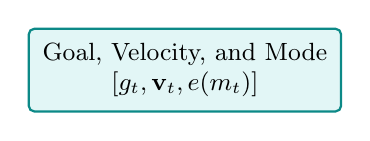
\begin{tikzpicture}
    \node[smallblock=pvoCyan, minimum width=3.60cm, minimum height=1.05cm]
        at (1.80,0.48) {Goal, Velocity, and Mode\\$[g_t,\mathbf v_t,e(m_t)]$};
\end{tikzpicture}

% 03: LiDAR temporal encoder.
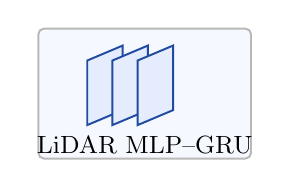
\begin{tikzpicture}
    \node[frame, fill=pvoBlue!5, minimum width=2.70cm, minimum height=1.65cm]
        at (1.35,0.83) {};
    \foreach \x in {0.62,0.94,1.26}{
        \draw[fill=pvoBlue!13, draw=pvoBlue!68!black, line width=0.7pt]
            (\x,0.43) -- ++(0.45,0.19) -- ++(0,0.82) -- ++(-0.45,-0.19) -- cycle;
    }
    \node[font=\small] at (1.35,0.18) {LiDAR MLP--GRU};
\end{tikzpicture}

% 04: State encoder.
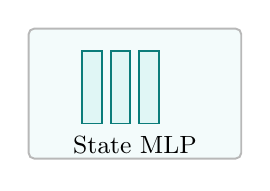
\begin{tikzpicture}
    \node[frame, fill=pvoCyan!5, minimum width=2.70cm, minimum height=1.65cm]
        at (1.35,0.83) {};
    \foreach \x in {0.68,1.04,1.40}{
        \draw[fill=pvoCyan!13, draw=pvoCyan!68!black, line width=0.7pt]
            (\x,0.45) rectangle ++(0.25,0.92);
    }
    \node[font=\small] at (1.35,0.18) {State MLP};
\end{tikzpicture}

% 05: Fused embedding.

\begin{tikzpicture}
    \draw[rounded corners=1.5pt, fill=pvoCyan!24, draw=pvoCyan!75!black,
          line width=1.0pt] (0.38,0) rectangle (0.92,3.25);
    \node[rotate=90, font=\bfseries\small, text=pvoCyan!55!black]
        at (0.65,1.62) {$e_t$};
\end{tikzpicture}

% 06: TD3 Actor.
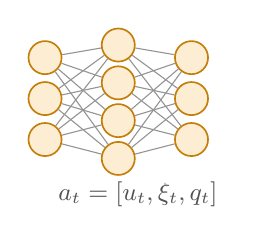
\begin{tikzpicture}
    \foreach \y [count=\i] in {1.92,1.40,0.88}
        \node[actor] (a1-\i) at (0.42,\y) {};
    \foreach \y [count=\j] in {2.08,1.60,1.12,0.64}
        \node[actor] (a2-\j) at (1.35,\y) {};
    \foreach \y [count=\k] in {1.92,1.40,0.88}
        \node[actor] (a3-\k) at (2.28,\y) {};
    \foreach \i in {1,...,3} \foreach \j in {1,...,4}
        \draw[thinlink] (a1-\i) -- (a2-\j);
    \foreach \j in {1,...,4} \foreach \k in {1,...,3}
        \draw[thinlink] (a2-\j) -- (a3-\k);
    \node[font=\small, text=black!68] at (1.60,0.18)
        {$a_t=[u_t,\xi_t,q_t]$};
\end{tikzpicture}

% 07: TD3 Critic.
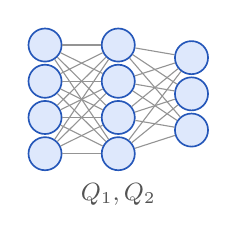
\begin{tikzpicture}
    \foreach \y [count=\i] in {2.08,1.62,1.16,0.70}
        \node[critic] (c1-\i) at (0.42,\y) {};
    \foreach \y [count=\j] in {2.08,1.62,1.16,0.70}
        \node[critic] (c2-\j) at (1.35,\y) {};
    \foreach \y [count=\k] in {1.92,1.46,1.00}
        \node[critic] (c3-\k) at (2.28,\y) {};
    \foreach \i in {1,...,4} \foreach \j in {1,...,4}
        \draw[thinlink] (c1-\i) -- (c2-\j);
    \foreach \j in {1,...,4} \foreach \k in {1,...,3}
        \draw[thinlink] (c2-\j) -- (c3-\k);
    \node[font=\small, text=black!68] at (1.35,0.18) {$Q_1,Q_2$};
\end{tikzpicture}

% 08: Neural-PVO risk head.
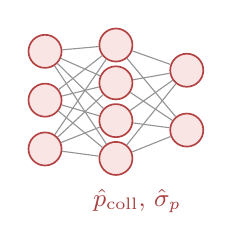
\begin{tikzpicture}
    \foreach \y [count=\i] in {2.08,1.46,0.84}
        \node[risk] (r1-\i) at (0.38,\y) {};
    \foreach \y [count=\j] in {2.16,1.68,1.20,0.72}
        \node[risk] (r2-\j) at (1.28,\y) {};
    \foreach \y [count=\k] in {1.84,1.08}
        \node[risk] (r3-\k) at (2.18,\y) {};
    \foreach \i in {1,...,3} \foreach \j in {1,...,4}
        \draw[thinlink] (r1-\i) -- (r2-\j);
    \foreach \j in {1,...,4} \foreach \k in {1,...,2}
        \draw[thinlink] (r2-\j) -- (r3-\k);
    \node[font=\small, text=pvoRed!75!black] at (1.55,0.18)
        {$\hat p_{\mathrm{coll}},\,\hat\sigma_p$};
\end{tikzpicture}

% 09: Safety filter.
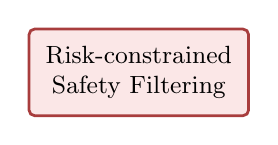
\begin{tikzpicture}
    \node[block=pvoRed, minimum width=2.60cm, minimum height=1.10cm]
        at (1.30,0.58) {Risk-constrained\\Safety Filtering};
\end{tikzpicture}

% 10: 4WIS action mapper.
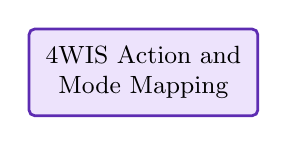
\begin{tikzpicture}
    \node[block=pvoPurple, minimum width=2.90cm, minimum height=1.10cm]
        at (1.45,0.58) {4WIS Action and\\Mode Mapping};
\end{tikzpicture}

% 11: Safe body velocity.
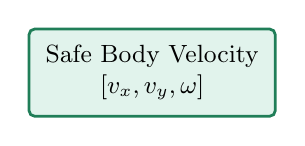
\begin{tikzpicture}
    \node[block=pvoGreen, minimum width=3.10cm, minimum height=1.10cm]
        at (1.55,0.58) {Safe Body Velocity\\$[v_x,v_y,\omega]$};
\end{tikzpicture}

% 12: Geometric proxy.

\begin{tikzpicture}
    \node[smallblock=pvoGray, minimum width=4.50cm, minimum height=0.72cm,
          font=\small] at (2.25,0.42)
        {Current: clearance + rollout + UQ proxy};
\end{tikzpicture}

% 13: IRSim training scene.
\begin{tikzpicture}
    \node[draw=pvoBlue!65!black, line width=1.0pt, inner sep=2pt]
        at (1.65,1.35)
        {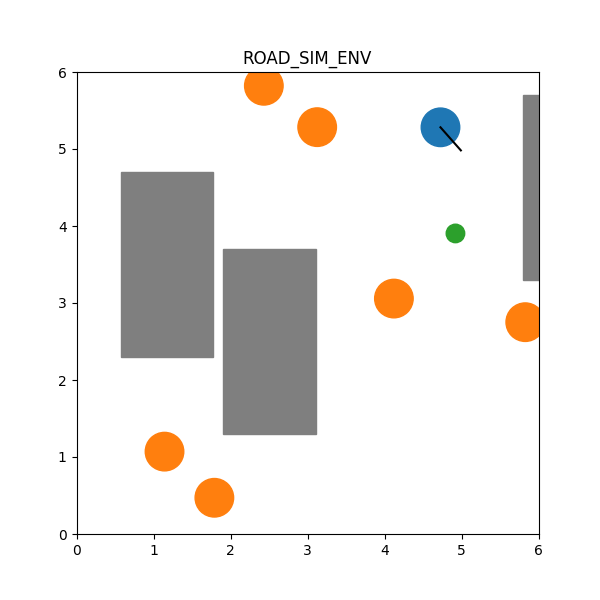
\includegraphics[width=3.30cm,height=2.10cm]{../../images/irsim_frame.png}};
\end{tikzpicture}

% 14: Reward and transition.
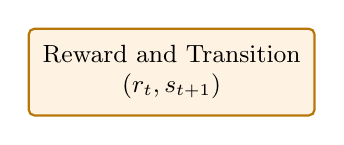
\begin{tikzpicture}
    \node[smallblock=pvoOrange, minimum width=2.90cm, minimum height=1.10cm]
        at (1.45,0.58) {Reward and Transition\\$(r_t,s_{t+1})$};
\end{tikzpicture}

% 15: Gazebo validation scene.
\begin{tikzpicture}
    \node[draw=pvoGreen!65!black, line width=1.0pt, inner sep=2pt]
        at (1.78,1.35)
        {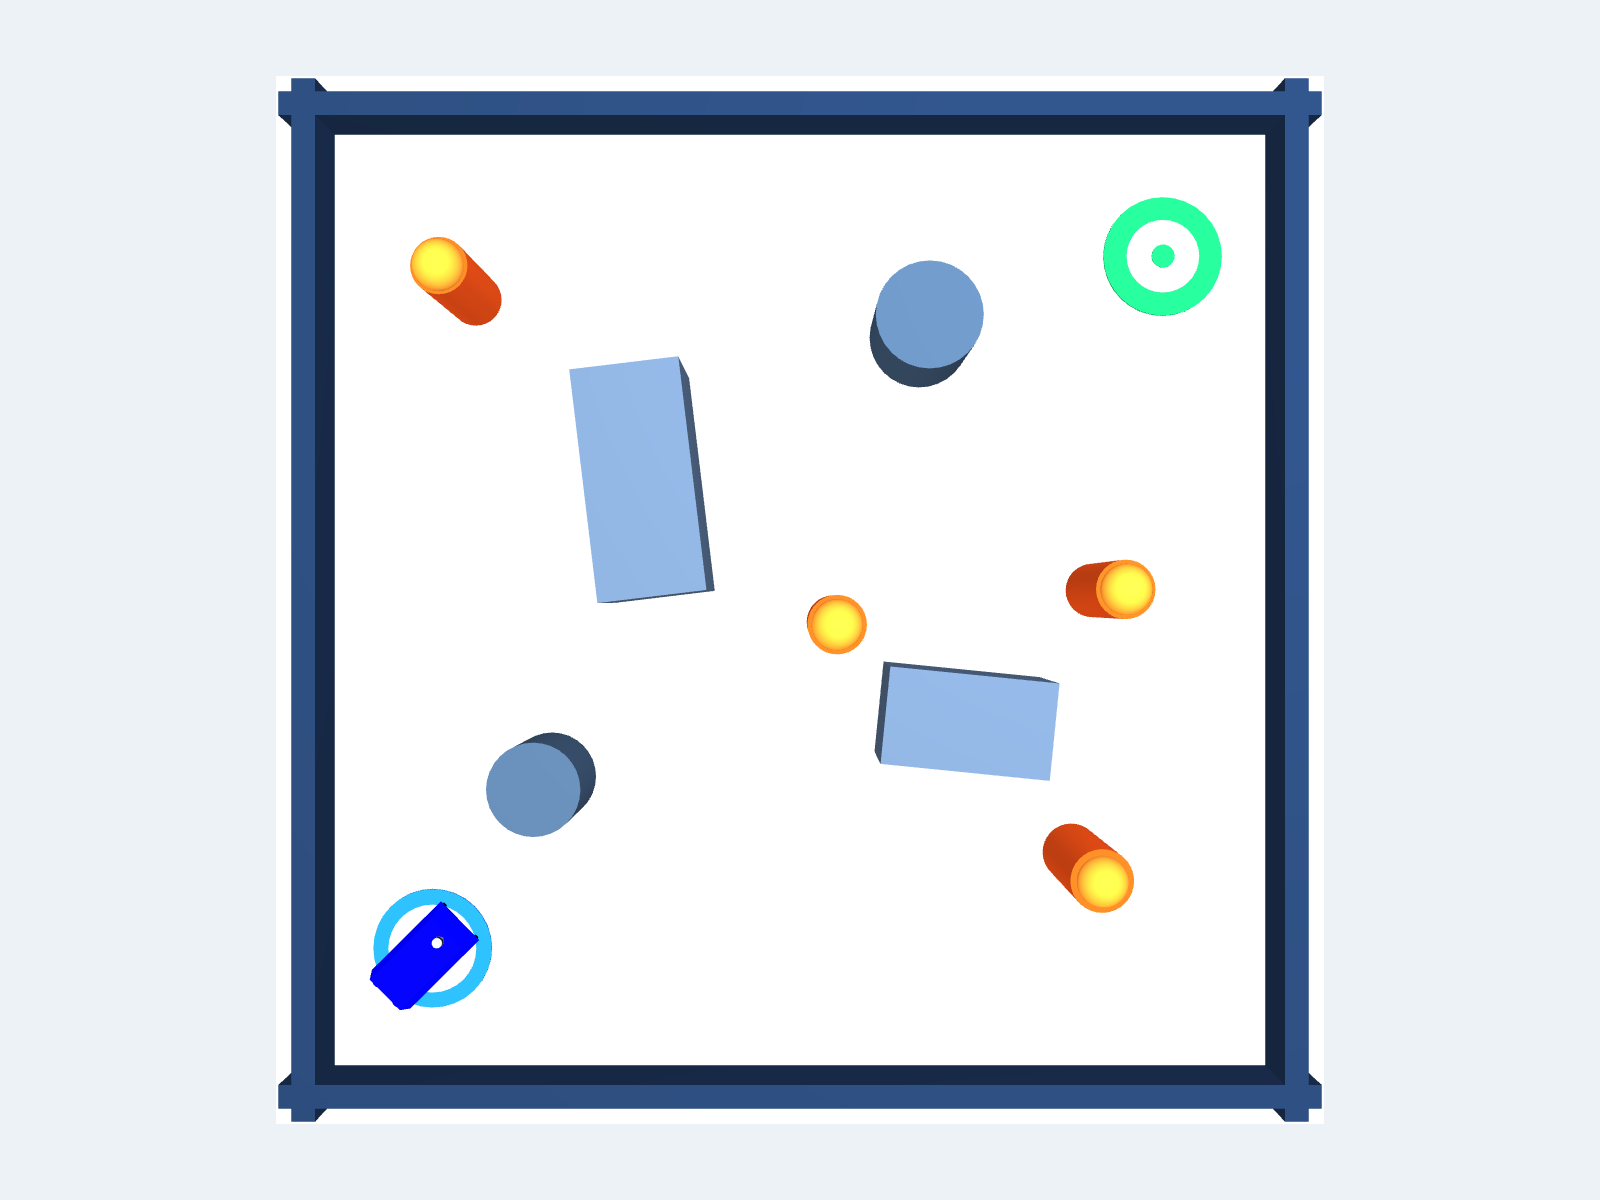
\includegraphics[width=3.55cm,height=2.10cm]{../../images/gazebo_neural_pvo_overview.png}};
\end{tikzpicture}

\end{document}
